\documentclass[a4paper]{article}

\usepackage[english]{babel}
\usepackage[utf8]{inputenc}
\usepackage{algorithm}
\usepackage[noend]{algpseudocode}
\usepackage{amsmath}
\usepackage{amssymb}
\usepackage{filecontents}
\usepackage{cite}
\usepackage{graphicx}

\DeclareMathOperator*{\argmin}{arg\,min}
\title{Research Plan}
\author{Myeong-Jang Pyeon\and Yu-Min Kim\and Hak-Su Lim}
\begin{filecontents*}{\jobname.bib}

%%%%%%%%%%%%%%%%%%%%%%%%%%%%%%%%%%%%%

@inproceedings{vidal2005probabilistic,
  title={Probabilistic finite-state machines-part I},
  author={Vidal, Enrique and Thollard, Franck and De La Higuera, Colin and Casacuberta, Francisco and Carrasco, Rafael C},
  journal={IEEE transactions on pattern analysis and machine intelligence},
  volume={27},
  number={7},
  pages={1013--1025},
  year={2005},
  publisher={IEEE}
}

@inproceedings{vidal2005probabilistic2,
  title={Probabilistic finite-state machines-part II},
  author={Vidal, Enrique and Thollard, Frank and De La Higuera, Colin and Casacuberta, Francisco and Carrasco, Rafael C},
  journal={IEEE Transactions on Pattern Analysis and Machine Intelligence},
  volume={27},
  number={7},
  pages={1026--1039},
  year={2005},
  publisher={IEEE}
}

@inproceedings{de2013most,
  title={The most probable string: an algorithmic study},
  author={De La Higuera, Colin and Oncina, Jos{\'e}},
  journal={Journal of Logic and Computation},
  volume={24},
  number={2},
  pages={311--330},
  year={2013},
  publisher={Oxford University Press}
}

@inproceedings{de2004learning,
  title={Learning stochastic finite automata},
  author={De La Higuera, Colin and Oncina, Jos{\'e}},
  booktitle={International Colloquium on Grammatical Inference},
  pages={175--186},
  year={2004},
  organization={Springer}
}

@inproceedings{de2013computing,
  title={Computing the most probable string with a probabilistic finite state machine},
  author={De La Higuera, Colin and Oncina, Jos{\'e}},
  booktitle={Proceedings of the 11th International Conference on Finite State Methods and Natural Language Processing},
  pages={1--8},
  year={2013}
}

@inproceedings{cognetta2018online,
  title={Online Stochastic Pattern Matching},
  author={Cognetta, Marco and Han, Yo-Sub},
  booktitle={International Conference on Implementation and Application of Automata},
  pages={121--132},
  year={2018},
  organization={Springer}
}

@book{de2010grammatical,
  title={Grammatical inference: learning automata and grammars},
  author={De La Higuera, Colin},
  year={2010},
  pages={99--132},
  publisher={Cambridge University Press}
}
@inproceedings{ballespectral,
  title={Spectral learning techniques for weighted automata, transducers, and grammars},
  author={De La Higuera, Colin and Oncina, Jos{\'e}},
  booktitle={Proceedings of Conference on Empirical Methods in Natural Language Processing  (EMNLP)},
  year={2014},
}


%%%%%%%%%%%%%%%%%%%%%%%%%%%%%%%%%%%%%%%%%%%%%%%%%%%%

\end{filecontents*}
\immediate\write18{bibtex \jobname}
\bibliographystyle{plain}
\begin{document}
\maketitle
\begin{center}
{
\large 
\textbf{Team Name:} Practical PFA (PPFA) \\
\textbf{Advisor:} Prof. Yo-Sub Han \\
\textbf{TA:} Marco Cognetta \\
\par 
}
\end{center}

\section{Probabilistic Finite-State Automata}
There are DFA/NFA that represent the accepting model to verify the acceptance of the strings, but if the probabilities is added to the transitions of the automata \cite{vidal2005probabilistic, vidal2005probabilistic2}. 
\textit{A}=$\langle\Sigma,Q,\mathbb{I_P},\mathbb{F_P},\delta_\mathbb{P}\rangle$ this is called PFA and represents the string generating model. The PFA satisfies the following conditions.\\
\begin{quotation}
\noindent
- $Q$ is a finite set of states; these will be labelled $q_1,\dots, q_{|Q|}$ unless otherwise stated\\
- $\Sigma$ is the alphabet\\
- $\mathbb{I_P}$ : Q $\rightarrow$ $\mathbb{Q^+}$ $\cap$ [0, 1] \textit{(initial-state probabilities)}\\
- $\mathbb{F_P}$ : Q $\rightarrow$ $\mathbb{Q^+}$ $\cap$ [0, 1] \textit{(final-state probabilities)}\\
- $\delta_\mathbb{P}$ : Q $\times$ ($\Sigma \cup \{\lambda\}$) $\times$ Q $\rightarrow$ $\mathbb{Q^+}$ \textit{is a transition function; the function is complete:} $\delta_\mathbb{P}$ \textit{(q,a,q') = 0 can be interpreted as "no transition from $q$ to $q'$ labelled with a". We will also denote $(q,a,q',P)$ instead of $\delta_\mathbb{P}(q,a,q') = P$ where P is a probability.}\\ 
\end{quotation}
$\mathbb{I_P}$, $\mathbb{\delta_P}$ and $\mathbb{F_P}$ are functions such that:\\
\begin{align*}
\sum_{q\in\textit{Q}}\mathbb{I_P}(q) = 1, \\
\end{align*}
\begin{align*}
and \enspace\forall q \in \textit{Q}, \mathbb{F_P}(q)+\sum_{a\in\sum\cup\{\lambda\}, q'\in\textit{Q}}\delta_\mathbb{P}(q,a,q') = 1.\\
\end{align*}
\\If the PFA generates a string, the string has a probability of being generated by the PFA. We can also find the distributions in which the strings are generated through string sampling. The distribution satisfies the following conditions.\\
\begin{quotation}
\noindent
-\textit{$Pr_D(x)$} is the probability of a string \textit{x} $\in$ $\Sigma^*$ under the distribution \textit{D} \\
-$\sum_{\textit{x}\in\Sigma^*}$ \textit{$Pr_D(x)$} = 1. \\
-$\forall q \in Q$, $\mathbb{F_P}(q)$ + $\sum_{a \in \Sigma\cup\{\lambda\}, q' \in Q}\delta_\mathbb{P}(q,a,q') = 1.$ \\
\end{quotation}
If $\lambda$-transitions are added to the PFA it is called a $\lambda$-PFA.
The PFA can be represnted with graph. Figure 1 is an example of the graph of the PFA \cite{de2010grammatical}. The numbers on the left of the state name are initial probabilities and the numbers on the right of the state name are final probabilities. The number on the 
transitions are transition probabilities. For example, the probability of parsing string "ab" with this PFA is  
\textit{$Pr_A(ab)$} that
\begin{align*}
Pr_A(ab)&= \mathbb{I_P}(q_1)\cdot\delta_\mathbb{P}(q_1,a,q_2)\cdot\delta_\mathbb{P}(q_2,b,q_4)\cdot\mathbb{F_P}(q_4)\nonumber\\
&\quad +\mathbb{I_P}(q_2)\cdot\delta_\mathbb{P}(q_2,a,q_3)\cdot\delta_\mathbb{P}(q_3,b,q_3)\cdot\mathbb{F_P}(q_3)\\
&\quad +\mathbb{I_P}(q_2)\cdot\delta_\mathbb{P}(q_2,a,q_3)\cdot\delta_\mathbb{P}(q_3,b,q_4)\cdot\mathbb{F_P}(q_4) \\
&= 0.4\cdot0.5\cdot0.4\cdot0.3\\
&\quad + 0.6\cdot0.5\cdot0.2\cdot0.4\\
&\quad + 0.6\cdot0.5\cdot0.4\cdot0.3 \\
&= 0.084
\end{align*}
\begin{figure}[htbp]
\begin{center}
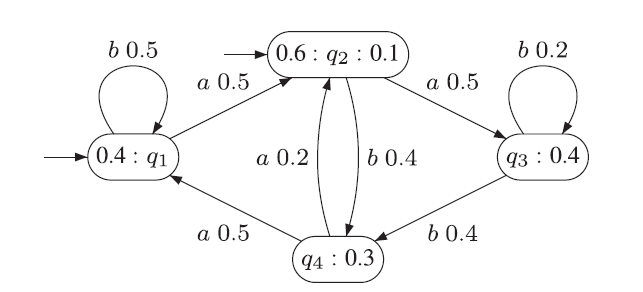
\includegraphics[scale=0.7]{figure1}
\caption{Graphical representation of a PFA \cite{de2010grammatical}} \label{fig:label}
\end{center}
\end{figure}



%%
\section{Problems}
\subsection{Related Problems}
In probabilistic automata theory, an important question is what the most probable string is. Without any constraint, the problem is called as the \textit{consensus string} problem. The formal definition is as below.\\
\textbf{Name:} Consensus string (Cs) \\
\textbf{Instance:} A probabilistic machine $\mathcal{M}$ \\
\textbf{Question:} Find in $\Sigma^{*}$ a string $x$ such that $\forall y\in \Sigma^{*}, {Pr}_{\mathcal{M}}(x) \geq {Pr}_{\mathcal{M}}(y)$.
\newline
\par
This problem can be modified as a decision problem. It is called as the \textit{most probable string} problem, defined as below. \\
\textbf{Name:} Most probable string (MPS) \\
\textbf{Instance:} A probabilistic machine $\mathcal{M}$ and $p\geq 0$ \\
\textbf{Question:} Find in $\Sigma^{*}$ a string $x$ such that ${Pr}_{\mathcal{M}}(x) > p$.
\newline
\par
If an extra constraint for the length of strings is added, it is called as the \textit{bounded most probable string} problem, which is defined as below. \\
\textbf{Name:} Bounded most probable string (BMPS)\\
\textbf{Instance:} A probabilistic machine $\mathcal{M}$, $p\geq 0$, and an integer $b$ \\
\textbf{Question:} Find in $\Sigma^{\leq b}$ a string $x$ such that ${Pr}_{\mathcal{M}}(x) > p$.
\par
\subsection{Our Problem}
In this project, we will solve another problem. In our setting, we are given a string so that the solution space is reduced to the set of string within $k-$distance with the given string. We call it as the \textit{most probable string within $k-$distance} problem and the formal definition is described as below. \\
\textbf{Name:} Most probable string within $k-$distance \\
\textbf{Instance:} A probabilistic machine $\mathcal{M}$, $p\geq 0$, a string $w$, and $k\in \mathbb{N}$ \\
\textbf{Question:} Find in $\Sigma^{*}$ a string $x$ such that ${Pr}_{\mathcal{M}}(x) > p$ and dist($x$, $w$)$\leq k$.\\
Note that the solution space is a subset of $\Sigma^{\leq |w|+k}$. So, it is not necessary to add the constraint for the length of strings.
\newline

\section{Previous Research}
% The MPS problem and the decision problem of it are NP-hard
% Suggest the bounded decision problem (BMPS) for the decision problem (NP-hard?)
% There exist a psuedo-polynomial exact algorithm to solve BMPS with PFA. (not to general probabilistic machine)

The problem of finding the most probable string (MPS) for a distribution generated by a probabilistic finite-state automaton is NP-hard.\cite{de2013most, de2013computing} Therefore the decision problem of it, which determines whether there exist a string whose probability on this machine is bigger than a given probability p, is also NP-hard. The one main reason is that there is no bound on the string. The most probable string can be of exponential length.\cite{de2013most, de2013computing}\\

We focus on the bounded decision problem of MPS(BMPS). In that case, there is an additional input integer b that bounds the length of the string lower than or equal to b. There is a pseudo-polynomial exact algorithm to solve BMPS.\cite{de2013most, de2013computing}\\

The problem we're interested in is MPS where distance within $k$ ($k$-MPS). Note that $k$-MPS is inherently a kind of BMPS because the length of string is bounded by edit(or hamming) distance $k$. There is an exact algorithm suggested by Marco Cognetta that solve this problem in pseudo-polynomial time when $k$ is lower than or equal to 1. However this algorithm cannot solve the problem in pseudo-polynomial time when $k$ is bigger than 1. We'll brainstorm how to efficiently solve $k$-MPS when $k$ is bigger than 2.

\section{Approaches}
As we mentioned above, there is no efficient algorithm to solve $k$-MPS. Therefore we expect to design such an efficient algorithm for $k$-MPS. What we have to do first is obtaining a PFA $\mathcal{M}^{'}$ that generates strings $w$ which can be generated by the original PFA $\mathcal{M}$ and satisfy dist($w$, $w_{0}$) $\leq k$. If we successfuly obtain $\mathcal{M}^{'}$, then we can reduce the problem to an instance of MPS.
However, the existing algorithm for MPS is psudo-polynomial, not strictly efficient. In fact, the time compleity of it is proportional to ${1} \over {p}$. Therefore, there are some challenges to do this,
\begin{itemize}
\item \textbf{Obtaining $\mathcal{M}^{'}$.} How to obtain $\mathcal{M}^{'}$ in polynomial time.
\item \textbf{MPS on $\mathcal{M}^{'}$.} We have two options, one is to use the existing pseudo-polynomial approximation  algorithm\cite{de2013most}, and the other is to invent a new polynomial approximation algorithm.
\end{itemize}


\section{Contribution}
If we solve k-MPS, we expect below applications \cite{cognetta2018online},
\begin{itemize}
\item \textbf{Spell Correction.} Since PFA is a generative model which generates distribution, we can obtain a PFA over a person's chat, for instance, from Kakao Talk. We expect to correct wrong sentences given the PFA and the algorithm that solve k-MPS. For example, we can easily correct a sentence "I am a toy", which is obviously wrong sentence, to "I am a boy".
\item \textbf{Image/Audio Reconstruction.} If we have a PFA on some image dataset like ImageNet, we can reconstruct(or restore) a broken image to normal one.
\end{itemize}

\section{Implementation}
\begin{figure}[htbp]
\begin{center}
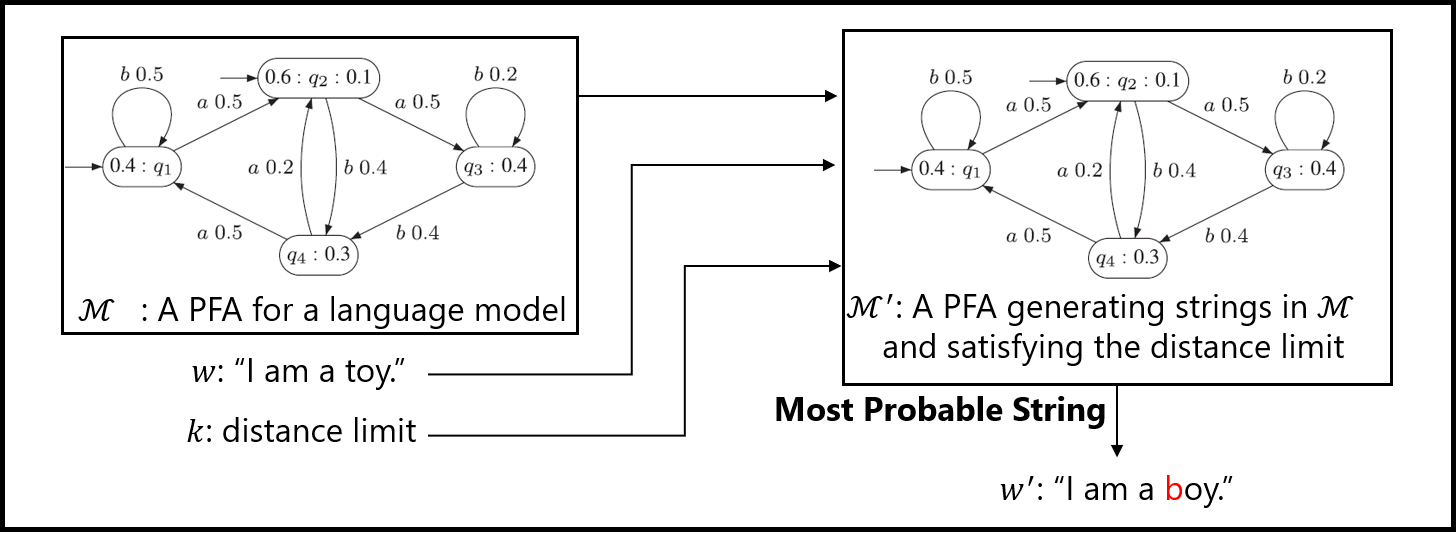
\includegraphics[scale=0.48]{implementation}
\caption{Graphical representation of Spell Correction using PFA and $k$-MPS} \label{fig:label}
\end{center}
\end{figure}

As an application of $k$-MPS, we will implement a spell correction algorithm. In order to do this, we first design a PFA framework. On the framework we learn a PFA for language modeling using spectral learning \cite{ballespectral}. The overall architecture for this implementation is illustrated in Figure 2.

\section{Role Division}
\begin{itemize}
\item \textbf{Yu-Min Kim.} 
\begin{itemize}
\item Design and implement the algorithm
\item Implement forward steps in the PFA framework
\end{itemize}
\item \textbf{Myeong-Jang Pyeon.} 
\begin{itemize}
\item Design and implement the algorithm
\item Implement the learning algorithm for PFA
\end{itemize}
\item \textbf{Yu-Min Kim.} 
\begin{itemize}
\item Design and implement the algorithm
\item Implement the GUI in the PFA framework
\end{itemize}
\end{itemize}

\section{Schedule}
Below is our schedule of this project.\\
\\
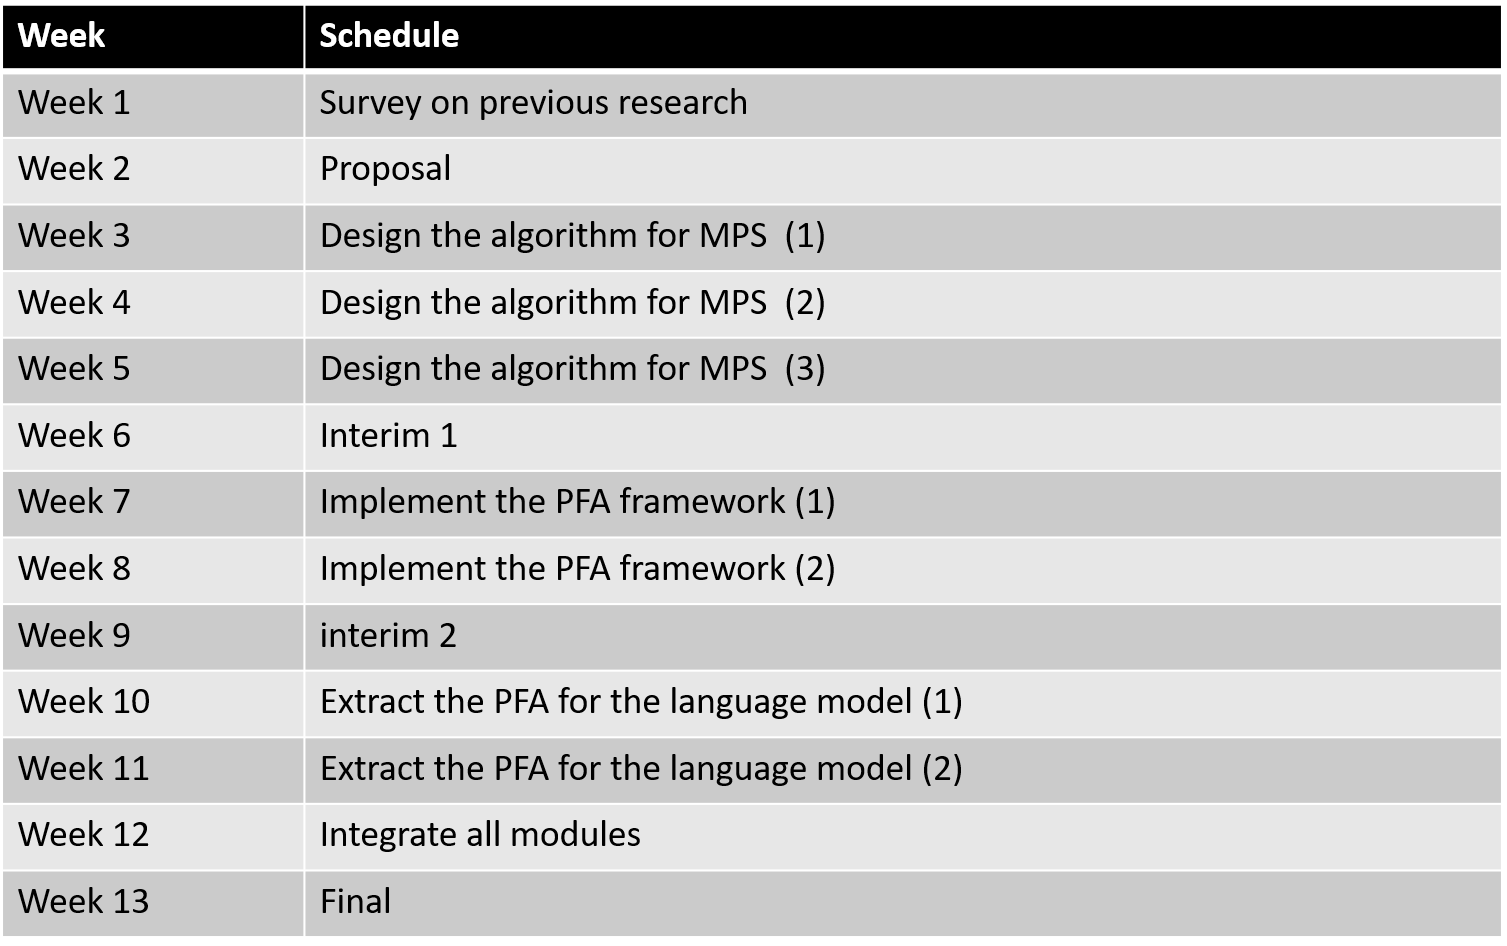
\includegraphics[scale=0.48]{schedule}


\bibliography{\jobname}

\end{document}